% figures/detect/fig_pca_scree.tex — loads PDF exported from NB03
% Requires \usepackage{graphicx}. Export the scree plot from NB03 as
% figures/detect/pca_scree.pdf (or .png and change the extension).
\begin{figure}[!ht]
    \centering
    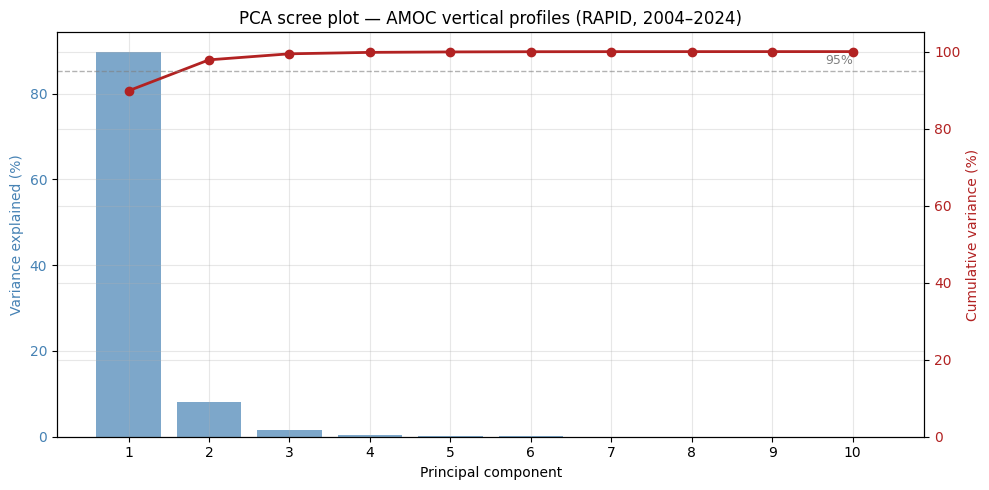
\includegraphics[width=0.8\textwidth]{figures/data_pipeline/pca_scree.png}
    \caption[Variance explained by the vertical PCA modes.]{\textbf{The vertical
    variability of the AMOC is almost one-dimensional.} Variance explained by each
    principal component of the 307-level vertical profiles. The first mode alone
    explains \SI{89.82}{\percent} and the first two together \SI{97.86}{\percent};
    the sharp elbow after the second mode marks where structure gives way to noise.
    This is the two-coordinate latent space the experiential representation is
    built on.}
    \label{fig:pca-scree}
\end{figure}
